\section{Sensorik}
Da wie oben beschrieben die Sensorik eine große Rolle im Bereich der IoT spielt, sind in diesem Kapitel die Grundlagen der Sensorik aufgeführt.  
\subsection{Allgemein}
Der Begriff \textit{Sensorik} kommt aus dem Latein. \textit{Sensus} bedeutet "der Sinn". Generell lässt sich sagen, dass ein Sensor ein System ist, das eine physikalische Größe und deren Änderung misst und die Messung in nutzbare Signale wandelt. 
Regelungen können Sensoren als Messerichtungen nutzen.  

\begin{figure}
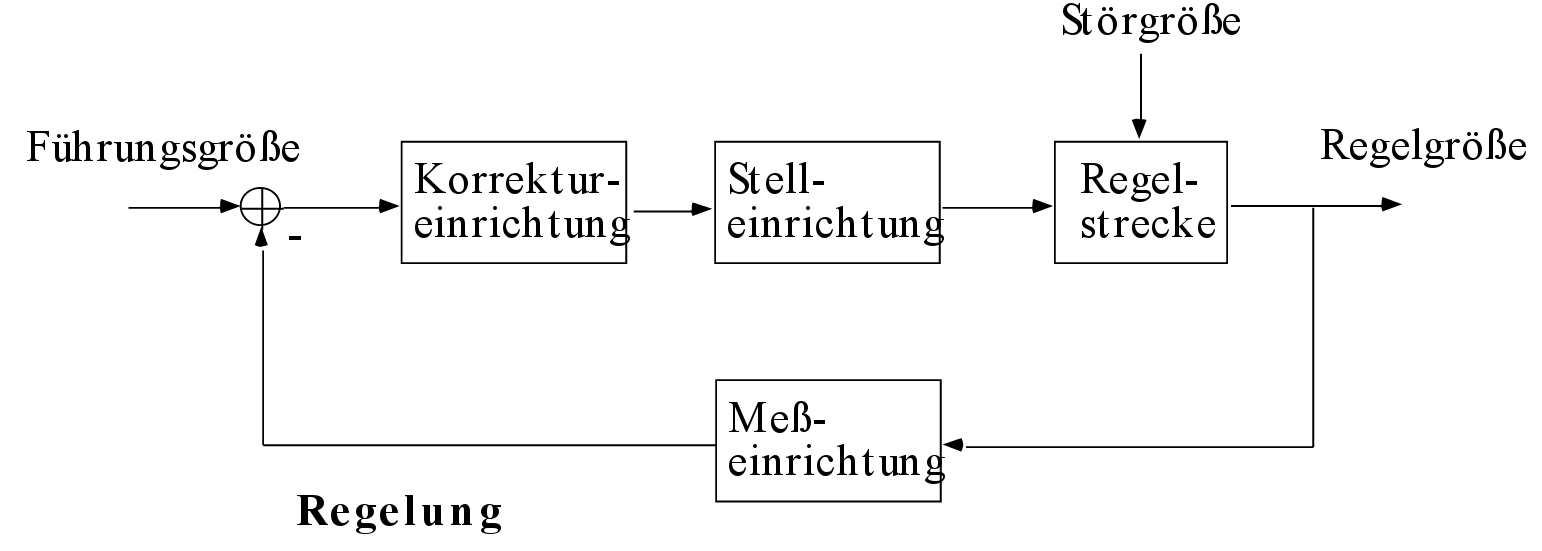
\includegraphics[scale=0.3
]{bilder/regelung} 
\caption[Schema einer Regelung]{Schema einer Regelung \cite{strand}}
\label{IPv4}
\end{figure}

Sensoren kann man in folgende Kategorien einteilen:
\begin{itemize}
\item Mechanische Sensoren
\item Temperatursensoren 
\item Chemische Sensoren
\item Biosensoren
\item Optische Sensoren 
\item Akustische Sensoren
\item Magnetische Sensoren 
\item Gassensoren
\end{itemize}

Mechanische Sensoren können beispielsweise Kontaktsensoren sein. Sie können zum benutzt werden um zu erkennen, ob eine Tür geschlossen ist. Chemische Sensoren können chemische Stoffe quantifizieren. Der Unterschied zu Biosensoren ist, dass diese meist organische Verbindungen messen können (zum Beispiel Glucose). 

Sensoren können unterschiedlich Komplex sein, je nach Anwendungsgebiet. Man unterscheidet zwischen:
\begin{itemize}
\item Elementarsensoren
\item Integrierten Sensoren
\item und Intelligenten Sensoren.
\end{itemize}

Elementare Sensoren sind man einfachsten aufgebaut. Im Falle eines optischen Sensors kann dieser aus leidlich einer Photozelle bestehen. Das Signal das er zurück gibt, muss unter Umständen ein A/D-Wandler noch digitalisieren. 
Ein Integrierter Sensor ist da schon komplexer. Er bereitet sein Signal auf. Das kann beispielsweise eine Verstärkung oder eine Filterung sein. Bei einem Intelligenten Sensor redet man schon von einem Rechner. Es kann sich zum Beispiel um eine Kamera oder um einen Laserscanner handeln. Derartige Sensoren arbeiten mit einer umfassenden Vorverarbeitung der Daten. 
Ferner unterscheidet man zwischen internen und externen Sensoren. Im weiteren betrachten wir die externen Sensoren. Sie sind in der IoT-Welt von hoher Bedeutung.
\cite{strand}
\subsection{Temperatur}
\begin{figure}
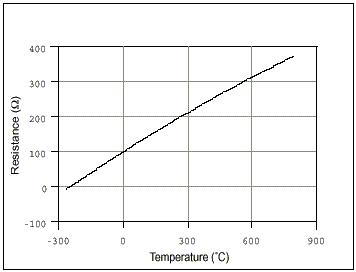
\includegraphics[scale=1]{bilder/pt100} 
\caption[PT100 Temperatursensor]{PT100 Temperatursensor \cite{pt100} }
\label{PT100}
\end{figure}
Die Temperatur lässt sich auf viel Art und Weisen berechnen. Sensoren für Mikrocontroller kann man in zwei Kategorien einteilen:
\begin{itemize}
\item Analoge Sensoren
\item Digitale Sensoren
\end{itemize}
Ein gängiger analoger Temperatursensor ist der \textit{PT100}. Es handelt sich hierbei um einen Platinwiderstand. Er hat bei null Grad Celsius einen Widerstand von 100 Ohm. Der Widerstand nimmt ungefähr 0,4 Ohm pro einem Grad Temperaturänderung zu. Ein Vorteil dieses Sensors ist es, dass er einen großen Messbereich hat. Generell benötigt man für derartige Temperatursensoren eine relativ komplexe Schaltung. Außerdem kann kann man mit dem Sensor einen relativ großen Temperaturbereich abdecken.

\cite{mc2}

\subsection{Luftfeuchtigkeit}
\label{sec:Luftfeute}
Luftfeutigkeitssensoren messen meist die relative Luftfeuchte. Dazu benutzen moderne Messeinrichtgen entweder;
\begin{itemize}
\item kapazitive oder 
\item widerstandsbasierte Verfahren.
\end{itemize}
Bei der kapazitiven Messung ist ein Kondensator vorhanden.  Die Dielektrizitätskonstante ändert sich in Abhängigkeit von der Luftfeuchte. Damit ändert sich auch die Kapazität des Kondensators. Über eine Messung der Kapazität kann man auf die Luftfeuchte schließen.
Bei einem anderen Verfahren nutzt man Materialien deren Leitfähigkeit abhängig von der Luftfeuchte ist. Mit einer Widerstandsmessung kann man dann auf die Luftfeuchte schließen.



\subsection{Beleuchtungsstärke}
Zur Helligkeitsmessung kann man entweder Photowiderstände oder Photohalbleiter verwenden. 
Der ohmsche Widerstand eines Photowiderstandes ist abhängig vom einfallenden Licht. Über eine Widerstandsmessung kann man dann über auf die Helligkeit schließen. 
Photohalbleiter induzieren bei einfallendem Licht eine Spannung.

\begin{figure}
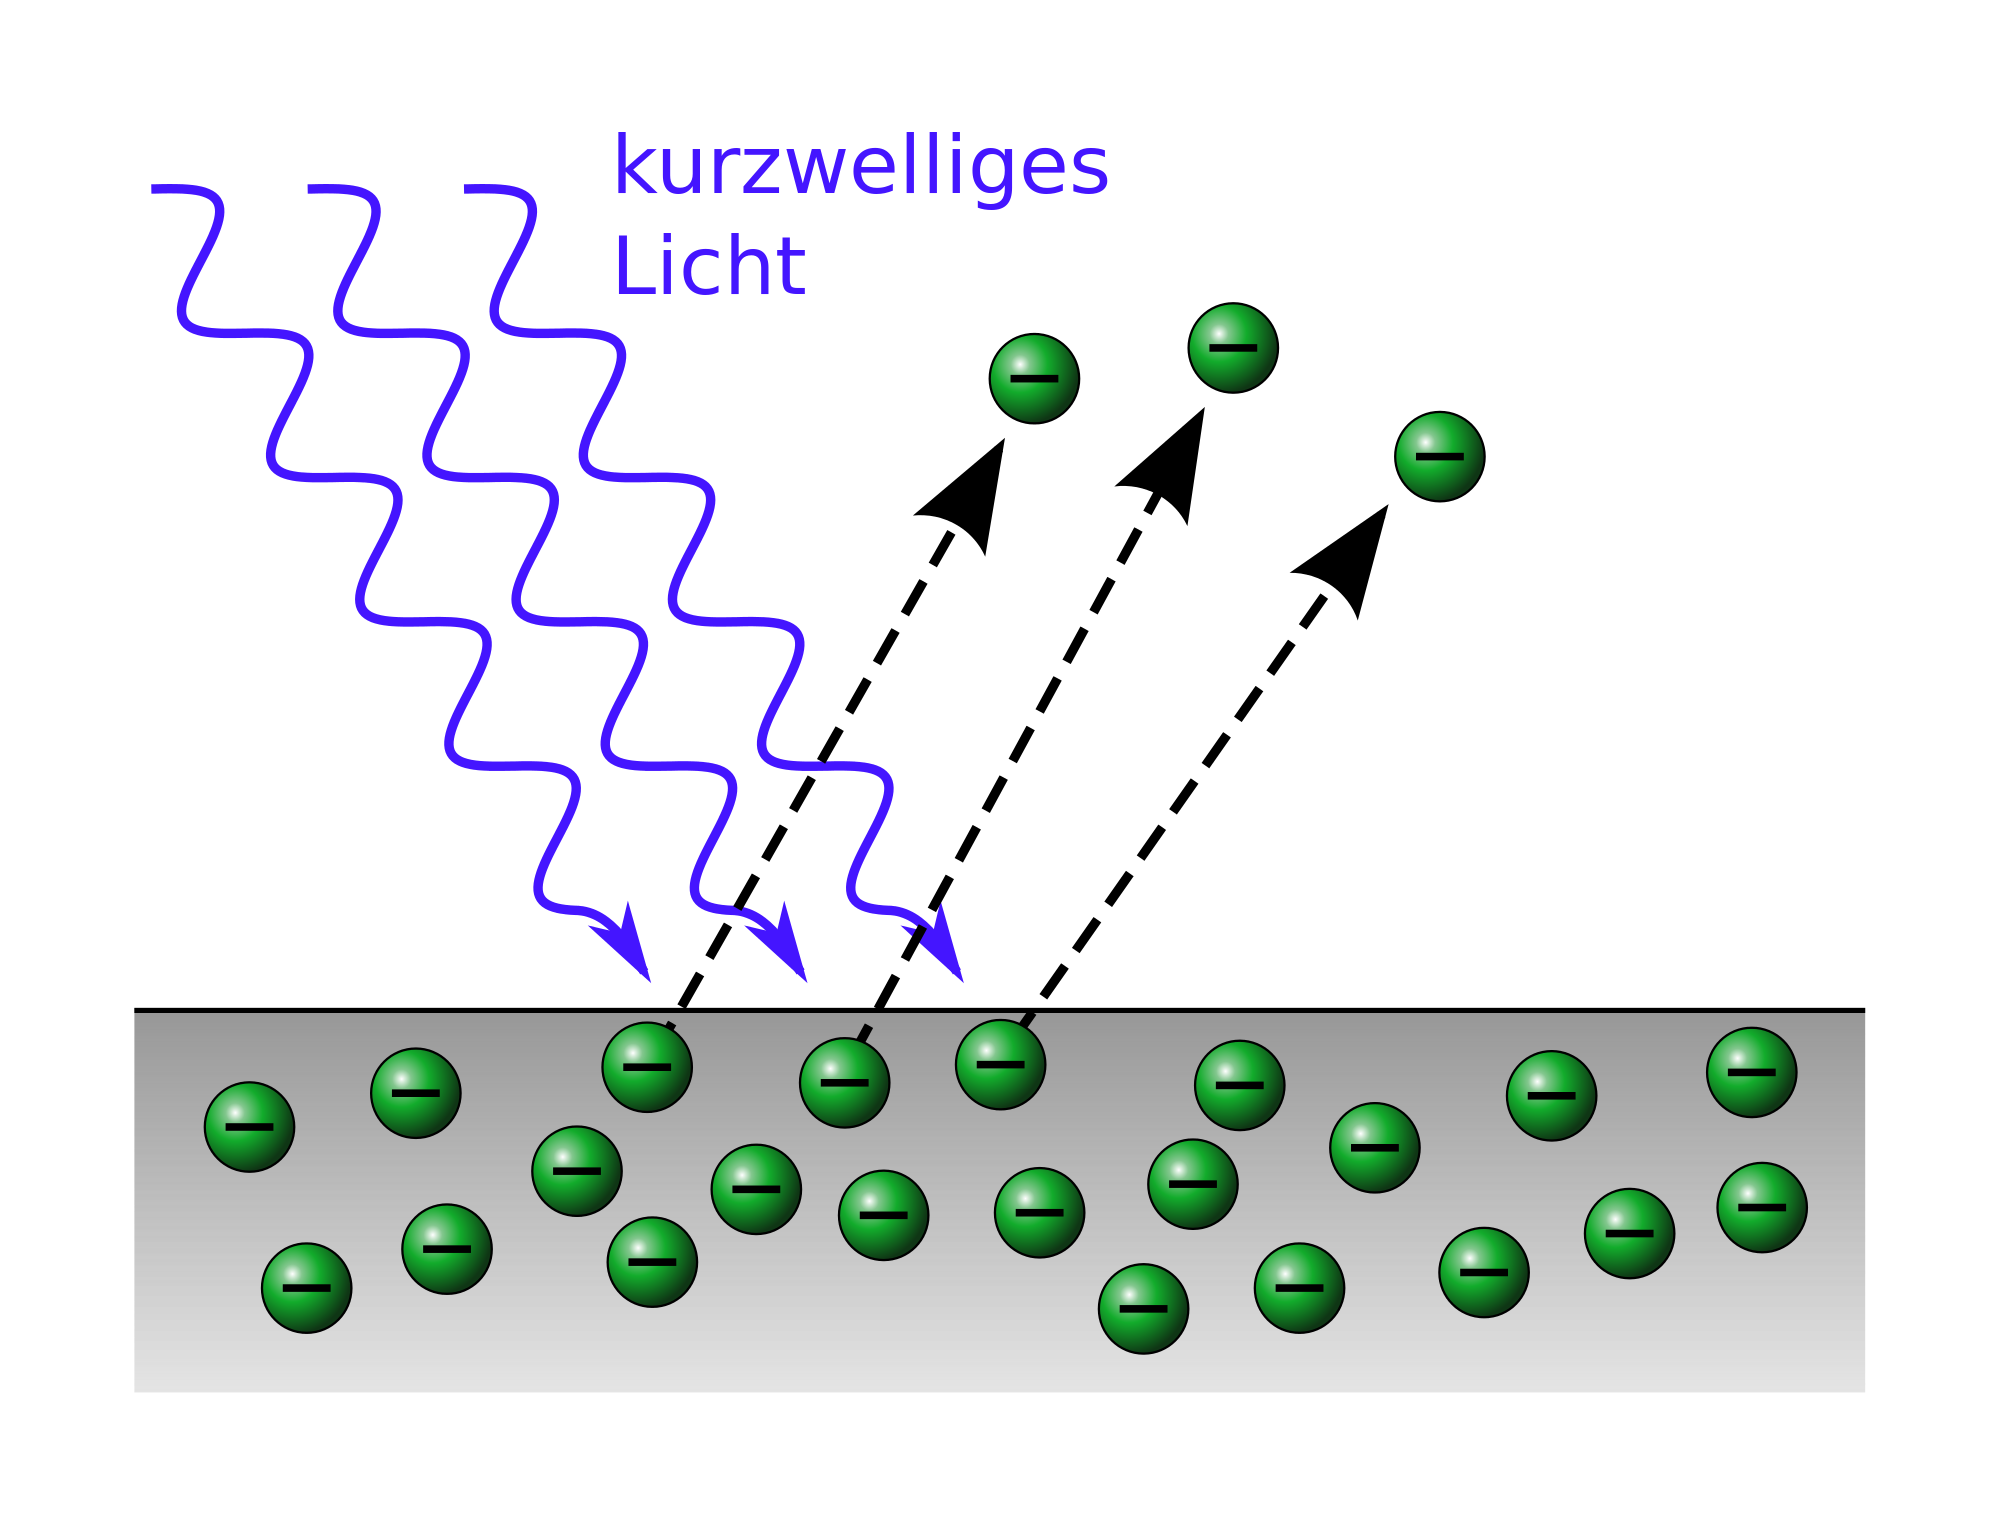
\includegraphics[scale=0.1]{bilder/Fotoelektrischer_Effekt} 
\caption[Photoelektrischer Effekt]{Photoelektrischer Effekt \cite{wikiPhoto} }
\label{Bewegungsmelder}
\end{figure}

Einfallende Photonen regen Elektronen in der Photozelle an. Die Bewegung der Elektronen kann man als Spannung messen.

\cite{mc}

\subsection{Bewegungsmelder}
\begin{figure}
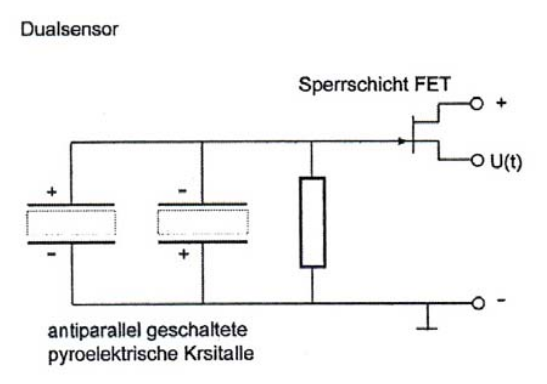
\includegraphics[scale=0.4]{bilder/bewegungsmelder} 
\caption[Schaltplan eines IR-Bewegungsmelders]{Schaltplan eines IR-Bewegungsmelders \cite{UniMuenchen}}
\label{Bewegungsmelder}
\end{figure}
Bewegungsmelder können mit Infrarotstrahlung arbeiten. Sie messen die Infrarotstrahlung und geben zurück, sobald sich diese ändert. 
Die Sensoren nutzen dazu den pyroelektrischen Effekt. In Bewegungsmelder kommen zwei dieser Sensoren zum Einsatz.   



Ein pyroelektrischer Sensor kann man nun direkt in einen Raum richten, beispielsweise mithilfe einer Linse. Verdeckt ein Objekt den einen Sensor, löschen sich nun die Spannungen der pyroelektrischen Bauteuile nicht mehr aus. Der Bewegungsmelder gibt zurück, dass er eine Bewegung erkannt hat. 

\cite{UniMuenchen}

\subsection{Luftdruck}
Den atmosphärischen Luftdruck kann man mit Absolutdrucksensoren messen. Die Messerichtungen haben ein Vakuum. Das Vakuum trennt man mit einer Membran von der Umgebung. Ändert sich nun der Umgebungsdruck, so bewegt sich die Membran. Die Bewegung nutzt man, um mit Piezokristallen eine Spannung zu messen. Die Spannung ist bei größeren Bewegungen und somit größeren Änderungen des Luftdrucks auch größer.

\begin{figure}
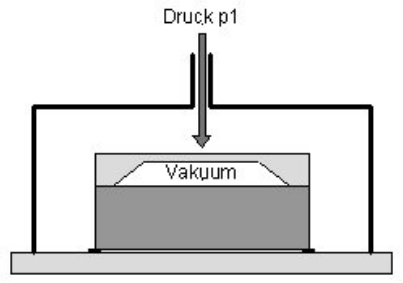
\includegraphics[scale=0.5]{bilder/drucksensor} 
\caption[Drucksensor]{Drucksensor}
\label{Drucksensor}
\end{figure}

\cite{Firstsensor}

\subsection{Bodenfeuchte}
Die Messung der Bodenfeuchte kann dem gleichen Prinzip wie die Messung der Luftfeuchte folgen (Kapitel \ref{sec:Luftfeute}). 


 
